\section{Mathematical Notation}
The ultimate goal of this research is to minimize the execution time of a parallel loop. Here is an example of a hpx for loop. 

\begin{figure*}[h]
	\centering
	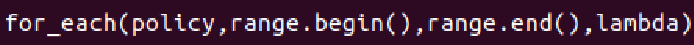
\includegraphics[scale=0.8]{images/for_each_call.pdf}
\end{figure*}

In such loops, a lambda function is applied over a range. The lambda function could be any algorithm such as,for instance, matrix multiplication. Each instance of a loop being run will be referred to as an experiment. Each experiment has an unique set of features which will be called $X_i$ for the $i$th experiment. The following six features are used:

\begin{itemize}
	\item[1] <Total Number of operations per iteration>
	\item[2] <Number of float operations per iteration>
	\item[3] <Number of comparison operations per iteration>
	\item[4] <Deepest loop level>
	\item[5] <Input size (range)>
	\item[6] <Number of threads>
\end{itemize}

The first four features will considered static since they only depend on the lambda function internal structure. They are collected at compile time by a ClangTool called loop convert.

The last two are dynamic since they do not depend on the algorithm and are extracted at run-time.

If we assume that the variance in time measurement is small, we can say that time is a function of features and chunk size. If the set of all possible features is denoted by $\{X_i\}$ and the set of all possible chunk sizes by $CS$ then we have:

$$t:\{X_i\} \otimes CS \rightarrow \mathbb{R}$$

$\otimes$ is a tensorial product which means that time is a function of both features and chunk size.
Our ultimate goal is to find the chunk size that minimizes the execution times for a given set of features. This means that we want to find the function:

\begin{equation}
	f(X_i)=cs_i
\end{equation}
 where
\begin{equation}
 cs_i=\underset{cs \in CS}{\arg\min} \, \, t(X_i,cs)
\end{equation}


The  value $cs_i$ is known as the optimal chunk size as it minimizes the execution time for experiment $i$. $f$ is the function that outputs the optimal chunk size of a given loop. Optimal chunk sizes will be referred to as target values which is the vocabulary used in machine learning for values that we want to predict.

The objective is to use machine-learning algorithms to approximate the function f (1) and (2).
